\documentclass[12pt, a4paper, onecolumn, oneside, final]{report}

\usepackage{uithesis}

%-----------------------------------------------------------------------------%
% Informasi Mengenai Dokumen
%-----------------------------------------------------------------------------%
% 
\usepackage{booktabs}
\usepackage{bigstrut}

\usepackage{colortbl}
\usepackage{etoolbox}
\patchcmd{\tableofcontents}{\@starttoc}{\vspace{-1cm}\@starttoc}{}{}
%-----------------------------------------------------------------------------%
\setlength{\parindent}{0em}
\setlength{\parskip}{1em}

% Judul laporan. 
\var{\judul}{DESAIN DAN SIMULASI
	PERLINDUNGAN PROPERTI INTELEKTUAL
	MENGGUNAKAN ALGORITME FILTER DIGITAL}
% 
% Tulis kembali judul laporan, kali ini akan diubah menjadi huruf kapital
\Var{\Judul}{DESAIN DAN SIMULASI
	PERLINDUNGAN PROPERTI INTELEKTUAL
	MENGGUNAKAN ALGORITME FILTER DIGITAL}
% 
% Tulis kembali judul laporan namun dengan bahasa Ingris
\var{\judulInggris}{DESIGN AND SIMULATION OF INTELECTUAL PROPERTIES PROTECTION
	USING DIGITAL FILTER ALGORITHM}

% 
% Tipe laporan, dapat berisi Skripsi, Tugas Akhir, Thesis, atau Disertasi
\var{\type}{Tugas Akhir}
% 
% Tulis kembali tipe laporan, kali ini akan diubah menjadi huruf kapital
\Var{\Type}{Tugas Akhir}
% 
% Tulis nama penulis 
\var{\penulis}{Hanjara Cahya Adhyatma}
% 
% Tulis kembali nama penulis, kali ini akan diubah menjadi huruf kapital
\Var{\Penulis}{Hanjara Cahya Adhyatma}
% 
% Tulis NPM penulis
\var{\npm}{1104131113}
% 
% Tuliskan Fakultas dimana penulis berada
\Var{\Fakultas}{Teknik Elektro}
\var{\fakultas}{Teknik Elektro}
% 
% Tuliskan Program Studi yang diambil penulis
\Var{\Program}{S1 Sistem Komputer}
\var{\program}{S1 Sistem Komputer}
% 
% Tuliskan tahun publikasi laporan
\Var{\bulanTahun}{2017}
% 
% Tuliskan gelar yang akan diperoleh dengan menyerahkan laporan ini
\var{\gelar}{S1 Sistem Komputer}
% 
% Tuliskan tanggal pengesahan laporan, waktu dimana laporan diserahkan ke 
% penguji/sekretariat
\var{\tanggalPengesahan}{XX Juli 2017} 
% 
% Tuliskan tanggal keputusan sidang dikeluarkan dan penulis dinyatakan 
% lulus/tidak lulus
\var{\tanggalLulus}{XX Januari 2010}
% 
% Tuliskan pembimbing 
\var{\pembimbing}{Prof. XXXX}
% 
% Alias untuk memudahkan alur penulisan paa saat menulis laporan
\var{\saya}{Penulis}

%-----------------------------------------------------------------------------%
% Judul Setiap Bab
%-----------------------------------------------------------------------------%
% 
% Berikut ada judul-judul setiap bab. 
% Silahkan diubah sesuai dengan kebutuhan. 
% 
\Var{\kataPengantar}{KATA PENGANTAR}
\Var{\babSatu}{Pendahuluan}
\Var{\babDua}{Tinjauan Pustaka}
\Var{\babTiga}{Desain dan Simulasi}
\Var{\babEmpat}{Pengujian dan Analisis}
\Var{\babLima}{Kesimpulan dan Saran}
\Var{\babEnam}{Apa Ya}
\Var{\kesimpulan}{Kesimpulan dan Saran}


%
% Hyphenation untuk Indonesia 
%
% @author  Andreas Febrian
% @version 1.00
% 
% Tambahkan cara pemenggalan kata-kata yang salah dipenggal secara otomatis 
% oleh LaTeX. Jika kata tersebut dapat dipenggal dengan benar, maka tidak 
% perlu ditambahkan dalam berkas ini. Tanda pemenggalan kata menggunakan 
% tanda '-'; contoh:
% menarik
%   --> pemenggalan: me-na-rik
%

\hyphenation{
    % alphabhet A
    a-na-li-sa a-tur 
    a-pli-ka-si 
    % alphabhet B
    ba-ngun-an 
    be-be-ra-pa 
    ber-ge-rak
    ber-ke-lan-jut-an 
    ber-pe-nga-ruh 
    % alphabhet C
    ca-ri
    % alphabhet D
    di-sim-pan di-pim-pin de-ngan da-e-rah di-ba-ngun da-pat di-nya-ta-kan 
    di-sim-bol-kan di-pi-lih di-li-hat de-fi-ni-si
    % alphabhet E
    e-ner-gi eks-klu-sif
    % alphabhet F
    fa-si-li-tas
    % alphabhet G
    ga-bung-an ge-rak
    % alphabhet H
    ha-lang-an
    % alphabhet I
    % alphabhet J
    % alphabhet K
    ke-hi-lang-an
    ku-ning 
    kua-li-tas ka-me-ra ke-mung-kin-an ke-se-pa-ham-an
    % alphabhet L
    ling-kung-an
    % alphabhet M
    me-neng-ah
    meng-a-tas-i me-mung-kin-kan me-nge-na-i me-ngi-rim-kan 
    meng-u-bah meng-a-dap-ta-si me-nya-ta-kan mo-di-fi-ka-si
    meng-a-tur
    % alphabhet N
    nya-ta non-eks-klu-sif
    % alphabhet O
    % alphabhet P
	pe-nye-rap-an 
	pe-ngon-trol
    pe-mo-del-an
    pe-ran  pe-ran-an-nya
    pem-ba-ngun-an pre-si-den pe-me-rin-tah prio-ri-tas peng-am-bil-an 
    peng-ga-bung-an pe-nga-was-an pe-ngem-bang-an 
    pe-nga-ruh pa-ra-lel-is-me per-hi-tung-an per-ma-sa-lah-an 
    pen-ca-ri-an peng-struk-tur-an
    % alphabhet Q
    % alphabhet R
    ran-cang-an
    % alphabhet S
    si-mu-la-si sa-ngat
    % alphabhet T
    te-ngah
    ter-da-pat
    % alphabhet U
    % alphabhet V
    % alphabhet W
    % alphabhet X
    % alphabhet Y
    % alphabhet Z
    % special
}

%
% @author  Andreas Febrian
% @version 1.00
% 
% Mendaftar seluruh istilah yang mungkin akan perlu dijadikan 
% italic atau bold pada setiap kemunculannya dalam dokumen. 
% 

\var{\license}{\f{Creative Common License 1.0 Generic}}
\var{\bslash}{$\setminus$}

\begin{document}

\begin{titlepage}
	\begin{center}
		\vspace*{1.0cm}
		% judul thesis harus dalam 14pt Times New Roman
		\bo{\Judul} \\[1.0cm]
		\bo{\textit{\judulInggris}} \\[1.0cm]  
		% harus dalam 14pt Times New Roman
		\bo{\Type} \\[1.0cm]
		% keterangan prasyarat
		\bo{Disusun sebagai syarat untuk memperoleh gelar Sarjana Teknik \\
			pada Program Studi \gelar\\
			Universitas Telkom}\\[1.0cm]
		\bo{Oleh}\\[1.0cm]
		% penulis dan npm
		\bo{\Penulis} \\
		\bo{\npm} \\
		
		\vspace*{1.0cm}
		\begin{figure}
			\begin{center}
				
\includegraphics[width=4.5cm]{pics/telu.png}
			\end{center}
		\end{figure}    
		\vspace*{0cm}
		% informasi mengenai fakultas dan program studi
		\bo{
			FAKULTAS \Fakultas\\
			Universitas Telkom \\
			Bandung \\
			\bulanTahun
		}
	\end{center}
\end{titlepage}

\pagenumbering{roman}

\addChapter{HALAMAN JUDUL}
\begin{titlepage}
	\begin{center}
		\vspace*{1.0cm}
		% judul thesis harus dalam 14pt Times New Roman
		\bo{\Judul} \\[1.0cm]
		\bo{\textit{\judulInggris}} \\[1.0cm]  
		% harus dalam 14pt Times New Roman
		\bo{\Type} \\[1.0cm]
		% keterangan prasyarat
		\bo{Disusun sebagai syarat untuk memperoleh gelar Sarjana Teknik \\
			pada Program Studi \gelar\\
			Universitas Telkom}\\[1.0cm]
		\bo{Oleh}\\[1.0cm]
		% penulis dan npm
		\bo{\Penulis} \\
		\bo{\npm} \\
		
		\vspace*{1.0cm}
		\begin{figure}
			\begin{center}
				
\includegraphics[width=4.5cm]{pics/telu.png}
			\end{center}
		\end{figure}    
		\vspace*{0cm}
		% informasi mengenai fakultas dan program studi
		\bo{
			FAKULTAS \Fakultas\\
			Universitas Telkom \\
			Bandung \\
			\bulanTahun
		}
	\end{center}
\end{titlepage}

\setcounter{page}{2}

\addChapter{LEMBAR PENGESAHAN}
\chapter*{HALAMAN PERSETUJUAN}

\vspace*{0.2cm}

\newpage

\addChapter{LEMBAR PERNYATAAN ORISINALITAS}
%
% Halaman Orisinalitas
%
% @author  Andreas Febrian
% @version 1.01
%

\chapter*{\uppercase{halaman pernyataan orisinalitas}}
\vspace*{2cm}

\begin{center}
	\bo{\type~ini adalah hasil karya saya sendiri, \\ 
	dan semua sumber baik yang dikutip maupun dirujuk \\
	telah saya nyatakan dengan benar.} \\
	\vspace*{2.6cm}
	
	\begin{tabular}{l c l}
	\bo{Nama} & : & \bo{\penulis} \\
	\bo{NPM} & : & \bo{\npm} \\ 
	\bo{Tanda Tangan} & : & \\
	& & \\
	& & \\
	\bo{Tanggal} & : & \bo{\tanggalPengesahan} \\	
	\end{tabular}
\end{center}

\newpage

\addChapter{ABSTRAK}
%
% Halaman Abstrak
%
% @author  Andreas Febrian
% @version 1.00
%

\chapter*{Abstrak}

\vspace*{0.2cm}

\noindent \begin{tabular}{l l p{10cm}}
	Nama&: & \penulis \\
	Program Studi&: & \program \\
	Judul&: & \judul \\
\end{tabular} \\ 

\vspace*{0.5cm}

\noindent \todo{Tuliskan abstrak laporan disini.} \\

\vspace*{0.2cm}

\noindent Kata Kunci: \\ 
\noindent \todo{Tuliskan kata kunci yang berhubungan dengan laporan 
	disini} \\

\newpage

\addChapter{ABSTRACT}
\chapter*{ABSTRACT}

\noindent System on a Chip (SoC) is an embedded system module
Has a certain functionality in a silicon chip board that can also be called
With Veri Large Scale Integration (VLSI). The owner of the SoC design has
Copyright over the system design that has been created. Fabless manufacturing is
How to mold a hardware module that is designer Integrated Circuit (IC)
Is Outsourching from outside the printing factory.

\vspace*{0.5cm}
\noindent Fabless manufacturing from IC design has gap design theft
When the design will be printed or when the project requires mutiple module
With various functions from various designers. Therefore every module is VLSI
From this chip designer requires proof of ownership from the designer or
Production company.

\vspace*{0.5cm}
\noindent In this study plans to make a verification of ownership design
With 2 dedicated verification keys ie Polygate as the primary key going
Activate the second key, and the second key will be active which process
Using a digital filter algorithm.

\vspace*{0.2cm}

\noindent \textbf{Keywords}: VLSI, Intellectual Property Protection, Digital Signal Processing, Polygate Watermark.

\newpage

\addChapter{\kataPengantar}
%-----------------------------------------------------------------------------%
\chapter*{\kataPengantar}
%-----------------------------------------------------------------------------%
Template ini disediakan untuk orang-orang yang berencana menggunakan 
\latex~untuk membuat dokumen tugas akhirnya. 
Mengapa \latex? 
Ada banyak hal mengapa menggunakan \latex, diantaranya:

\begin{enumerate}
	\item \latex~membuat kita jadi lebih fokus terhadap isi dokumen, bukan 
		tampilan atau halaman. 
	\item \latex~memudahkan dalam penulisan persamaan matematis. 
	\item Adanya automatis dalam penomoran caption, bab, subbab, subsubbab, 
		referensi, dan rumus. 
	\item Adanya automatisasi dalam pembuatan daftar isi, daftar gambar, dan
		daftar tabel. 
	\item Adanya kemudahan dalam memberikan referensi dalam tulisan dengan 
		menggunakan label. Cara ini dapat meminimalkan kesalahan pemberian 
		referensi. 
\end{enumerate}

Template ini bebas digunakan dan 
didistribusikan sesuai dengan aturan \license, yang secara sederhana berisi: 

\begin{figure}
	\centering
	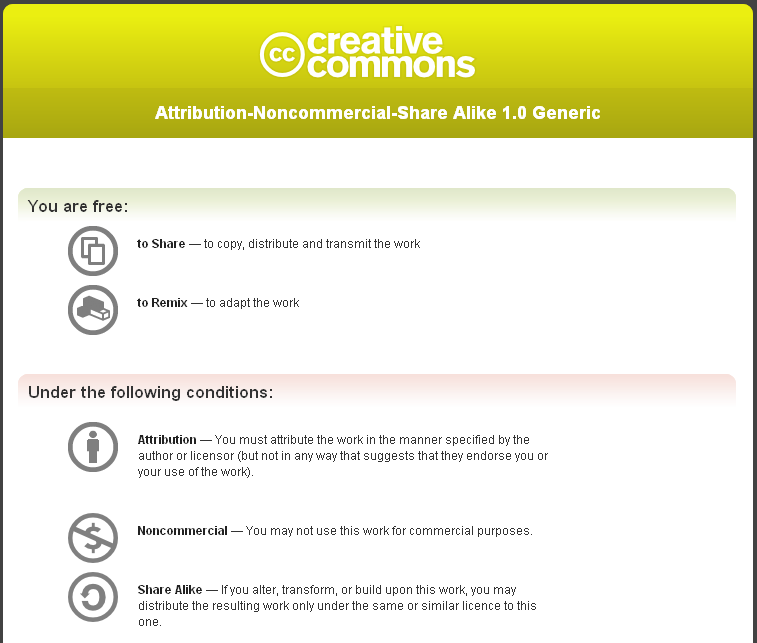
\includegraphics[width=0.74\textwidth]
		{pics/creative_common.png}
	\caption{\license}
	\label{fig:lisensi}
\end{figure}

\pic~\ref{fig:lisensi} diambil dari 
\url{http://creativecommons.org/licenses/by-nc-sa/1.0/deed.en_CA}. 
Jika ingin mengentahui lebih lengkap mengenai \license, silahkan buka 
\url{http://creativecommons.org/licenses/by-nc-sa/1.0/legalcode}. 
Seluruh dokumen yang dibuat dengan menggunakan template ini sepenuhnya 
menjadi hak milik pembuat dokumen dan bebas didistribusikan sesuai dengan 
keperluan masing-masing. 
Lisensi hanya berlaku jika ada orang yang membuat template baru dengan 
menggunakan template ini sebagai dasarnya. 

Dokumen ini dibuat dengan \latex~juga. Untuk meyakinkan Anda, coba lihat 
properti dari dokumen ini dan Anda akan menemukan bagian seperti 
\pic~\ref{fig:pdflatex}. 
Dokumen ini dimaksudkan untuk memberikan gambaran kepada Anda seperti apa 
mudahnya menggunakan \latex~dan juga memperlihatkan betapa bagus dokumen 
yang dihasilkan. 
Seluruh url yang Anda temukan dapat Anda klik. 
Seluruh referensi yang ada juga dapat diklik. 
Untuk mengerti template yang disediakan, Anda tetap harus membuka kode 
\latex~dan bermain-main dengannya. 
Penjelasan dalam PDF ini masih bersifat gambaran dan tidak begitu 
mendetail, dapat dianggap sebagai pengantar singkat. 
Jika Anda merasa kesulitan dengan template ini, mungkin ada baiknya 
Anda belajar sedikit dasar-dasar \latex. 

\begin{figure}
	\centering
	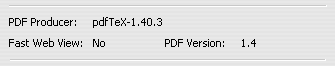
\includegraphics[width=0.54\textwidth]
		{pics/mark.png}
	\caption{Dokumen Dibuat dengan PDFLatex}
	\label{fig:pdflatex}
\end{figure}

Semoga template ini dapat membantu orang-orang yang ingin mencoba menggunakan 
\latex. Semoga template ini juga tidak berhenti disini dengan ada kontribusi 
dari para penggunanya. 
Kami juga ingin berterima kasih kepada Andreas Febrian, Lia Sadita, Fahrurrozi 
Rahman, Andre Tampubolon, dan Erik Dominikus atas kontribusinya dalam template 
ini. 

\vspace*{0.1cm}
\begin{flushright}
Depok, 30 Desember 2009\\[0.1cm]
\vspace*{1cm}
\penulis

\end{flushright}

\tableofcontents

\clearpage
\listoffigures
\clearpage
\listoftables
\clearpage

\addChapter{DAFTAR SINGKATAN}
\chapter*{DAFTAR SINGKATAN}

\addChapter{DAFTAR SIMBOL}
\chapter*{DAFTAR SIMBOL}

\addChapter{DAFTAR ISTILAH}
\chapter*{DAFTAR ISTILAH}

\addChapter{DAFTAR LAMPIRAN}
\chapter*{DAFTAR LAMPIRAN}

\pagenumbering{arabic}

%-----------------------------------------------------------------------------%
\chapter{\babSatu}
%-----------------------------------------------------------------------------%
\todo{tambahkan kata-kata pengantar bab 1 disini}


%-----------------------------------------------------------------------------%
\section{Latar Belakang}
%-----------------------------------------------------------------------------%
\todo{tuliskan latar belakang penelitian disini}


%-----------------------------------------------------------------------------%
\section{Permasalahan}
%-----------------------------------------------------------------------------%
Pada bagian ini akan dijelaskan mengenai definisi permasalahan 
yang \saya~hadapi dan ingin diselesaikan serta asumsi dan batasan 
yang digunakan dalam menyelesaikannya.


%-----------------------------------------------------------------------------%
\subsection{Definisi Permasalahan}
%-----------------------------------------------------------------------------%
\todo{Tuliskan permasalahan yang ingin diselesaikan. Bisa juga
	berbentuk pertanyaan}


%-----------------------------------------------------------------------------%
\subsection{Batasan Permasalahan}
%-----------------------------------------------------------------------------%
\todo{Umumnya ada asumsi atau batasan yang digunakan untuk 
	menjawab pertanyaan-pertanyaan penelitian diatas.}


%-----------------------------------------------------------------------------%
\section{Tujuan}
%-----------------------------------------------------------------------------%
\todo{Tuliskan tujuan penelitian.}


%-----------------------------------------------------------------------------%
\section{Posisi Penelitian}
%-----------------------------------------------------------------------------%
\todo{Posisi penelitian Anda jika dilihat secara bersamaan dengan 
	peneliti-peneliti lainnya. Akan lebih baik lagi jika ikut menyertakan 
	diagram yang menjelaskan hubungan dan keterkaitan antar 
	penelitian-penelitian sebelumnya}


%-----------------------------------------------------------------------------%
\section{Metodologi Penelitian}
%-----------------------------------------------------------------------------%
\todo{Tuliskan metodologi penelitian yang digunakan.}


%-----------------------------------------------------------------------------%
\section{Sistematika Penulisan}
%-----------------------------------------------------------------------------%
Sistematika penulisan laporan adalah sebagai berikut:
\begin{itemize}
	\item Bab 1 \babSatu \\
	\item Bab 2 \babDua \\
	\item Bab 3 \babTiga \\
	\item Bab 4 \babEmpat \\
	\item Bab 5 \babLima \\
	\item Bab 6 \babEnam \\
	\item Bab 7 \kesimpulan \\
\end{itemize}

\todo{Tambahkan penjelasan singkat mengenai isi masing-masing bab.}


%-----------------------------------------------------------------------------%
\chapter{\babDua}
%-----------------------------------------------------------------------------%

%-----------------------------------------------------------------------------%
\section{Pekerjaan Sebelumnya dan Keterkaitan}
%-----------------------------------------------------------------------------%
Secara garis besar teknik Intelectual Property Protection (IPP)
watermarking dapat diklasifikasikan menjadi 2 kelas yaitu Dynamic
Watermarking dan Static Watermarking. Dynamic Watermarking merupakan
watermark yang tidak dapat terdeteksi kecuali dengan menjalankan IP yang telah
di-watermark untuk mendeteksi sinyal yang dihasilkan, seperti digital signal
processing (DSP), atau finite state mechine (FSM) watermarking. Static
Watermarking merupakan watermark yang mengacu pada properti dari sebuah
desain, dan hanya bisa terdeteksi dengan cara statis yang berbeda, seperti jalur dan
penempatan watermarking [7].

Salah satu pengamanan lain adalah mengonversi fail simulasi dari fail.
RTL source code yang memungkinkan tidak mudah untuk di-reverse-engineering
oleh pihak ketiga, sehingga model tidak dapat dirubah dan digunakan kembali
dengan keperluan lain oleh pihak ketiga dan pengguna yang tidak bertanggung
jawab.[8][9]

Namun cara tersebut hanya melindungi dari sisi softwere yang melindungi
IP agar tidak di-salah-gunakan oleh pengguna pihak ketiga. Untuk pengamanan IP
yang digunakan dalam sharing project dan reusable project dapat digunakan
dengan pengamanan Digital Signal Processing cell yang memungkinkan integrasi
dalam sistem.

Dalam penelitian kali ini akan melakukan kombinasi dari proteksi IP
polimorph gate dengan algoritme filter digital. Menggunakan gabungan dari dua
teknik ini akan memberikan tambahan keamanan pada proteksi IP yang
kemungkinan tingkat over write watermark lebih kecil. Oleh karena itu dalam
penelitian ini mengajukan sebuah gabungan metode yang sudah ada untuk
meningkatkan kemampuan pengamanan dalam sebuah modul VLSI yang sudah
ada. Dengan menggabungkan polygate sebagai kunci kombinasi untuk
mengaktifkan modul filter digital yang akan digunakan sebagai watermark.

\section{Perancangan dan Implementasi Algoritme DSP untuk IPP}

Melakukan analisis terhadap masalah yang dikaji kemudian akan
dilakukan rancangan Intelectual Property Protection (IPP) dengan algoritme Filter
Digital yang dibangun meliputi rangkaian uji. Dari desain modul VLSI yang telah
ada akan diuji coba kan performa sebelum diberi watermark.

Dengan memberikan rangkaian watermark sebagai pengamanan pada
blueprint VLSI siap cetak yang menandakan kepemilikan dari desainer atau
perusahaan produsen modul akan melindungi dari kecurangan pihak lain yang
akan mencuri desain tersebut. Sehingga kemungkinan pencurian atau plagiarisme
berkurang yang menyebabkan kerugian pada perusahaan atau desainer karena
desain nya dicuri atau diplagiat.

Desain akan dirancang dengan kombinasi Low Pass Filter, High Pass
Filter, Band Pass Filter, dan Band Reject Filter. Kombinasi ini akan ditentukan
dan diaktifkan oleh polygate sebagai kunci pengaktifan kombinasi Filter digital.
Setelah Filter digital aktif maka kombinasi data akan melewati kombinasi filter
yang diaktifkan dari kombinasi polygate. Kemudian data hasil kombinasi proses
ini akan membentuk pola khusus yang menjadi data watermark dari desainer yang
mencirikan identitas desainer. Setelah diberikan watermark maka modul akan
diuji coba kan kembali performa nya. Bila terjadi penurunan performa maka akan
dilakukan perbaikan algoritma kemudian dilakukan diuji kembali performa nya.
Hingga didapat performa yang paling baik dari beberapa uji coba yang akan
dilakukan.

%-----------------------------------------------------------------------------%
\chapter{\babTiga}
%-----------------------------------------------------------------------------%
\todo{tambahkan kata-kata pengantar bab 1 disini}


%-----------------------------------------------------------------------------%
\section{Satu Persamaan}
%-----------------------------------------------------------------------------%

\noindent \begin{align}\label{eq:garis}
	\cfrac{y - y_{1}}{y_{2} - y_{1}} = 
	\cfrac{x - x_{1}}{x_{2} - x_{1}}
\end{align}

\equ~\ref{eq:garis} diatas adalah persamaan garis. 
\equ~\ref{eq:garis} dan \ref{eq:bola} sama-sama dibuat dengan perintah \bslash
align. 
Perintah ini juga dapat digunakan untuk menulis lebih dari satu persamaan. 

\noindent \begin{align}\label{eq:bola}
	\underbrace{|\overline{ab}|}_{\text{pada bola $|\overline{ab}| = r$}} 
		= \sqrt[2]{(x_{b} - x_{a})^{2} + (y_{b} - y_{a})^{2} + 
				\vert\vert(z_{b} - z_{a})^{2}}
\end{align}

%-----------------------------------------------------------------------------%
\section{Lebih dari Satu Persamaan}
\label{sec:multiEqu}
%-----------------------------------------------------------------------------%
\noindent \begin{align}\label{eq:matriks}	
	|\overline{a} * \overline{b}| &= |\overline{a}| |\overline{b}| \sin\theta 
		\\[0.2cm]
	\overline{a} * \overline{b} &=  
		\begin{array}{| c c c |}
			\hat{i} & x_{1} & x_{2} \\
			\hat{j} & y_{1} & y_{2} \\
			\hat{k} & z_{1} & z_{2} \\
		\end{array} \nonumber \\[0.2cm]
	&= \hat{i} \,
		\begin{array}{ | c c | }
			y_{1} & y_{2} \\
			z_{1} & z_{2} \\
		\end{array} 
	   + \hat{j} \,
		\begin{array}{ | c c | }
			z_{1} & z_{2} \\
			x_{1} & x_{2} \\
		\end{array} 
	   + \hat{k} \,	
		\begin{array}{ | c c | }
			x_{1} & x_{2} \\
			y_{1} & y_{2} \\
		\end{array}
		\nonumber
\end{align}

Pada \equ~\ref{eq:matriks} dapat dilihat beberapa baris menjadi satu bagian 
dari \equ~\ref{eq:matriks}. 
Sedangkan dibawah ini dapat dilihat bahwa dengan cara yang sama, \equ~
\ref{eq:gabungan1}, \ref{eq:gabungan2}, dan \ref{eq:gabungan3} memiliki nomor 
persamaannya masing-masing. 

\noindent \begin{align}\label{eq:gabungan1}	
	\int_{a}^{b} f(x)\, dx + \int_{b}^{c} f(x) \, dx = \int_{a}^{c} f(x) \, dx
		\\\label{eq:gabungan2}
	\lim_{x \to \infty} \frac{f(x)}{g(x)} = 0 \hspace{1cm} 
		\text{jika pangkat $f(x)$ $<$ pangkat $g(x)$} \\\label{eq:gabungan3}
	a^{m^{a \, ^{n}\log b }} = b^{\frac{m}{n}}
\end{align}


%-----------------------------------------------------------------------------%
\chapter{\babEmpat}
%-----------------------------------------------------------------------------%
\todo{tambahkan kata-kata pengantar bab 1 disini}

%-----------------------------------------------------------------------------%
\section{thesis.tex}
%-----------------------------------------------------------------------------%
Berkas ini berisi seluruh berkas Latex yang dibaca, jadi bisa dikatakan sebagai 
berkas utama. Dari berkas ini kita dapat mengatur bab apa saja yang ingin 
kita tampilkan dalam dokumen.


%-----------------------------------------------------------------------------%
\section{laporan\_setting.tex}
%-----------------------------------------------------------------------------%
Berkas ini berguna untuk mempermudah pembuatan beberapa template standar. 
Anda diminta untuk menuliskan judul laporan, nama, npm, dan hal-hal lain yang 
dibutuhkan untuk pembuatan template. 


%-----------------------------------------------------------------------------%
\section{istilah.tex}
%-----------------------------------------------------------------------------%
Berkas istilah digunakan untuk mencatat istilah-istilah yang digunakan. 
Fungsinya hanya untuk memudahkan penulisan.
Pada beberapa kasus, ada kata-kata yang harus selalu muncul dengan tercetak 
miring atau tercetak tebal. 
Dengan menjadikan kata-kata tersebut sebagai sebuah perintah \latex~tentu akan 
mempercepat dan mempermudah pengerjaan laporan. 


%-----------------------------------------------------------------------------%
\section{hype.indonesia.tex}
%-----------------------------------------------------------------------------%
Berkas ini berisi cara pemenggalan beberapa kata dalam bahasa Indonesia. 
\latex~memiliki algoritma untuk memenggal kata-kata sendiri, namun untuk 
beberapa kasus algoritma ini memenggal dengan cara yang salah. 
Untuk memperbaiki pemenggalan yang salah inilah cara pemenggalan yang benar 
ditulis dalam berkas hype.indonesia.tex.


%-----------------------------------------------------------------------------%
\section{pustaka.tex}
%-----------------------------------------------------------------------------%
Berkas pustaka.tex berisi seluruh daftar referensi yang digunakan dalam 
laporan. 
Anda bisa membuat model daftar referensi lain dengan menggunakan bibtex.
Untuk mempelajari bibtex lebih lanjut, silahkan buka 
\url{http://www.bibtex.org/Format}. 
Untuk merujuk pada salah satu referensi yang ada, gunakan perintah \bslash 
cite, e.g. \bslash cite\{latex.intro\} yang akan akan memunculkan 
\cite{latex.intro}


%-----------------------------------------------------------------------------%
\section{bab[1 - 6].tex}
%-----------------------------------------------------------------------------%
Berkas ini berisi isi laporan yang Anda tulis. 
Setiap nama berkas e.g. bab1.tex merepresentasikan bab dimana tulisan tersebut 
akan muncul. 
Sebagai contoh, kode dimana tulisan ini dibaut berada dalam berkas dengan nama 
bab4.tex. 
Ada enam buah berkas yang telah disiapkan untuk mengakomodir enam bab dari 
laporan Anda, diluar bab kesimpulan dan saran. 
Jika Anda tidak membutuhkan sebanyak itu, silahkan hapus kode dalam berkas 
thesis.tex yang memasukan berkas \latex~yang tidak dibutuhkan;  contohnya 
perintah \bslash include\{bab6.tex\} merupakan kode untuk memasukan berkas 
bab6.tex kedalam laporan.


%---------------------------------------------------------------
\chapter{\kesimpulan}
%---------------------------------------------------------------

%---------------------------------------------------------------
\section{Kesimpulan}
%---------------------------------------------------------------


%---------------------------------------------------------------
\section{Saran}
%---------------------------------------------------------------


%
% Daftar Pustaka 
% 

% 
% Tambahkan pustaka yang digunakan setelah perintah berikut. 
% 
\begin{thebibliography}{4}

\bibitem{latex.intro}
{Jeff Clark. (n.d). \f{Introduction to LaTeX}.
26 Januari 2010. \url{http://frodo.elon.edu/tutorial/tutorial/node3.html}.}

\end{thebibliography}



\begin{appendix}
	%
% @author  Andreas Febrian
% @version 1.00 
% 
% Hanya sebuah pembatas bertuliskan LAMPIRAN ditengah halaman. 
% 

\begin{titlepage}
	\centering 
	\vspace*{6cm}
	\noindent \Huge{LAMPIRAN}
	\addChapter{LAMPIRAN}
\end{titlepage}
	\setcounter{page}{2}
	%-----------------------------------------------------------------------------%
\addChapter{Lampiran 1}
\chapter*{Lampiran 1}
%-----------------------------------------------------------------------------%
\end{appendix}

\end{document}